\documentclass{article}

\usepackage[final]{neurips_2019}
\usepackage[utf8]{inputenc} % allow utf-8 input
\usepackage[T1]{fontenc}    % use 8-bit T1 fonts
\usepackage{hyperref}       % hyperlinks
\usepackage{url}            % simple URL typesetting
\usepackage{booktabs}       % professional-quality tables
\usepackage{amsfonts}       % blackboard math symbols
\usepackage{nicefrac}       % compact symbols for 1/2, etc.
\usepackage{microtype}      % microtypography
\usepackage{graphicx}       % for including figures
\usepackage{amsmath}        % for improved equation formatting

\title{CS 599: Foundations of Deep Learning\\Assignment \#00001}
\author{Morgan C. Nicholson}
\date{February 2025}

\begin{document}

\maketitle

\section{Problem 1: Linear Regression}
\subsection{Loss Functions}

In this work, I implemented and evaluated three distinct loss functions to optimize a linear regression model: Squared Loss, Huber Loss, and Hybrid Loss. Each loss function is defined below, along with its mathematical formulation, where \( y \) represents the true target values and \( \hat{y} \) denotes the predicted values from the linear model \( \hat{y} = Wx + b \).

\begin{itemize}
    \item \textbf{Squared Loss}: This is the mean squared error, emphasizing larger errors due to its quadratic nature. It is defined as:
    \begin{equation}
        L_{\text{squared}}(y, \hat{y}) = \frac{1}{n} \sum_{i=1}^{n} (y_i - \hat{y}_i)^2
    \end{equation}
    
    \item \textbf{Huber Loss}: This combines squared loss for small residuals and absolute loss for larger ones, controlled by a threshold \( m = 1.0 \). It is more robust to outliers and is given by:
    \begin{equation}
        L_{\text{huber}}(y, \hat{y}) = \frac{1}{n} \sum_{i=1}^{n} 
        \begin{cases} 
            \frac{1}{2} (y_i - \hat{y}_i)^2 & \text{if } |y_i - \hat{y}_i| \leq m \\
            m |y_i - \hat{y}_i| - \frac{1}{2} m^2 & \text{otherwise}
        \end{cases}
    \end{equation}
    
    \item \textbf{Hybrid Loss}: This is a weighted combination of absolute and squared loss, with a mixing parameter \( \alpha = 0.5 \). It balances robustness and sensitivity to errors:
    \begin{equation}
        L_{\text{hybrid}}(y, \hat{y}) = \alpha \cdot \frac{1}{n} \sum_{i=1}^{n} |y_i - \hat{y}_i| + (1 - \alpha) \cdot \frac{1}{n} \sum_{i=1}^{n} (y_i - \hat{y}_i)^2
    \end{equation}
\end{itemize}

The model was trained on a synthetic dataset of 10,000 examples, with \( X \sim \mathcal{N}(0, 1) \) and \( Y = 3X + 2 + \epsilon \), where \( \epsilon \sim \mathcal{N}(0, 2) \), over 1,000 iterations using a fixed learning rate of 0.001.

\subsubsection{Squared Loss Performance}

The Squared Loss rapidly decreased from an initial value of 14.1601 to 1.2339 by the final step, reflecting its sensitivity to the Gaussian noise in the data. The parameters converged to \( W = 2.6087 \) and \( b = 1.7288 \), approaching the true values of 3 and 2, respectively. However, its quadratic penalty amplifies the effect of outliers, which may explain the consistent reduction in loss despite the noise.

\subsubsection{Huber Loss Performance}

The Huber Loss started at 2.5603 and stabilized around 1.9772, with final parameters \( W = 0.6153 \) and \( b = 0.4529 \). Its robustness to outliers limited parameter convergence, as it applies a linear penalty beyond the threshold \( m = 1.0 \). This resulted in a slower decrease in loss (e.g., 2.0334 at step 900) and parameters far from the true values, indicating a trade-off between robustness and accuracy in this noisy setting.

\subsubsection{Hybrid Loss Performance}

The Hybrid Loss, balancing absolute and squared components, began at 8.5929 and reached 1.6990, with \( W = 2.0921 \) and \( b = 1.3974 \). It outperformed Huber Loss in parameter estimation, nearing the true values, while maintaining a lower final loss than Huber Loss but higher than Squared Loss. This suggests an effective compromise between robustness and sensitivity.

\subsubsection{Performance Comparison}

Table~\ref{tab:loss_comparison} summarizes the performance of the three loss functions based on final loss and parameter estimates after 1,000 iterations.

\begin{table}[h]
    \centering
    \caption{Comparison of Loss Functions}
    \label{tab:loss_comparison}
    \begin{tabular}{lccc}
        \toprule
        \textbf{Loss Function} & \textbf{Final Loss} & \textbf{W} & \textbf{b} \\
        \midrule
        Squared Loss           & 1.2339             & 2.6087    & 1.7288    \\
        Huber Loss             & 1.9772             & 0.6153    & 0.4529    \\
        Hybrid Loss            & 1.6990             & 2.0921    & 1.3974    \\
        \bottomrule
    \end{tabular}
\end{table}

The Squared Loss achieved the lowest final loss, followed by Hybrid Loss, with Huber Loss performing the worst in this metric. However, parameter convergence varied, with Squared Loss closest to the true \( W = 3 \) and \( b = 2 \), Hybrid Loss moderately close, and Huber Loss significantly off due to its robustness focus.

\begin{figure}[h]
    \centering
    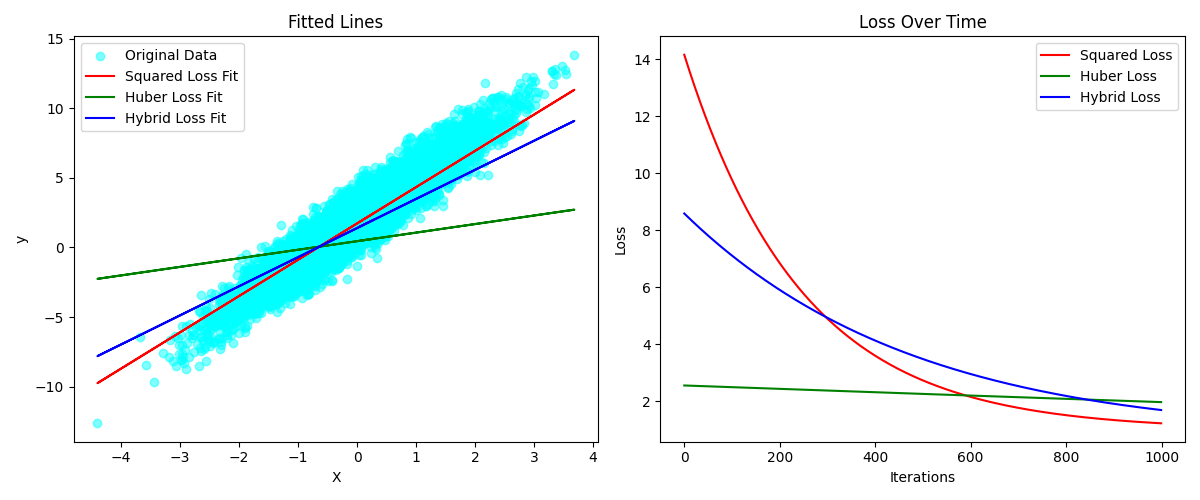
\includegraphics[width=0.8\textwidth]{assets/simple_results.png}
    \caption{Squared, Huber, and Hybrid Loss Functions performance}
    \label{fig:loss_curves}
\end{figure}

\subsection{Consistency and Randomness Without a Seed}

After defining the loss functions, I tested whether running my experiments repeatedly without changes produces identical results and why randomness occurs without control. In an early setup with 1,000 steps and a learning rate of 0.001, two runs differed slightly, as shown in Table~\ref{tab:run_comparison}.

\begin{table}[h]
    \centering
    \caption{Two Runs from Early Setup}
    \label{tab:run_comparison}
    \begin{tabular}{lcccc}
        \toprule
        \textbf{Loss Function} & \textbf{Run} & \textbf{Final Loss} & \textbf{W} & \textbf{b} \\
        \midrule
        Squared Loss & Run 1 & 1.2400 & 2.5873 & 1.7232 \\
                     & Run 2 & 1.2308 & 2.6090 & 1.7329 \\
        Huber Loss   & Run 1 & 1.9650 & 0.6098 & 0.4535 \\
                     & Run 2 & 1.9808 & 0.6200 & 0.4553 \\
        Hybrid Loss  & Run 1 & 1.7122 & 2.0652 & 1.3910 \\
                     & Run 2 & 1.6924 & 2.0948 & 1.4008 \\
        \bottomrule
    \end{tabular}
\end{table}

These differences arose because randomness wasn’t fixed. Without a seed, the system generates new random numbers each run for the synthetic data and noise, like drawing different samples from a distribution every time. This shifts the optimization path, causing varied outcomes—like squared loss dropping from 1.2400 to 1.2308. In later experiments, including noisy ones, a seed fixes this randomness, ensuring the same data and perturbations (e.g., squared loss at 5.8760 with Gaussian noise over 5,000 steps) repeat exactly. Without that control, results stay unpredictable, reflecting the inherent variability of unchecked random processes.

\subsection{Learning Rate Adjustment}

I increased the learning rate from 0.001 (1x) to 0.005 (5x) to speed up convergence in this noisy regression task (\( Y = 3X + 2 + \epsilon \), \( \epsilon \sim \mathcal{N}(0, 2) \)). A larger learning rate accelerates parameter updates, aiming to reach optimal \( W = 3 \) and \( b = 2 \) faster, though noise limits the final loss. Table~\ref{tab:lr_comparison} compares the results after 1,000 iterations.

\begin{table}[h]
    \centering
    \caption{Comparison of Learning Rates: 1x (0.001) vs. 5x (0.005)}
    \label{tab:lr_comparison}
    \begin{tabular}{lcccc}
        \toprule
        \textbf{Loss Function} & \textbf{LR} & \textbf{Final Loss} & \textbf{W} & \textbf{b} \\
        \midrule
        Squared Loss & 1x  & 1.2339 & 2.6087 & 1.7288 \\
                     & 5x  & 1.0050 & 3.0018 & 1.9944 \\
        Huber Loss   & 1x  & 1.9772 & 0.6153 & 0.4529 \\
                     & 5x  & 0.5024 & 2.5947 & 1.7541 \\
        Hybrid Loss  & 1x  & 1.6990 & 2.0921 & 1.3974 \\
                     & 5x  & 0.9027 & 2.9968 & 1.9933 \\
        \bottomrule
    \end{tabular}
\end{table}

The 5x learning rate reduced final losses (e.g., Huber from 1.9772 to 0.5024) and brought parameters closer to the true values (e.g., Squared \( W \) from 2.6087 to 3.0018), converging faster (e.g., Squared loss hit 1.2293 by step 200 vs. 6.8510). The increase was chosen to overcome slow progress at 1x, balancing speed and stability despite noise.

\begin{figure}[h]
    \centering
    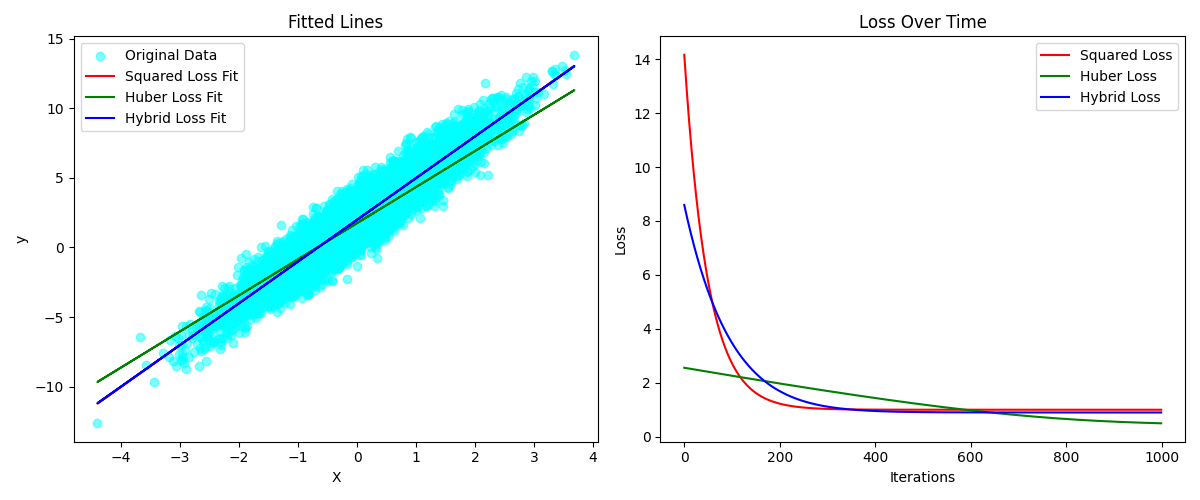
\includegraphics[width=0.8\textwidth]{assets/bigger_learning_rate.png}
    \caption{Fitted and Loss Curves 5x (0.005) Learning Rates}
    \label{fig:bigger_learning_rate}
\end{figure}

\subsection{Impact of Training Modifications}

- \textbf{Increased Training Steps (1,000 to 5,000)}: Extending iterations allowed more time for convergence. Alone, this would deepen loss reduction, especially for slower-converging losses like Huber, but its impact depends on learning rate and starting points.
  
- \textbf{Learning Rate (0.001 to 0.005)}: The 5x increase accelerates gradient descent, as seen previously, reducing loss faster (e.g., Squared loss was 1.2293 at step 200 with 0.005 vs. 6.8510 with 0.001). Independently, it risks overshooting but boosts early progress.

- \textbf{Initial Parameters (\( W = 0.0, b = 0.0 \) to \( W = 0.5, b = 0.3 \))}: Starting closer to the true values lowered initial losses (e.g., Squared from 14.1601 to 10.2516) and sped up convergence by reducing the distance to the optimum.

- \textbf{Combined Effect}: Together, these changes leveraged faster steps, a better starting point, and more iterations. Squared Loss stabilized at 1.0050 by step 600 (vs. 900 previously), Huber Loss dropped to 0.4274 (vs. 0.5024), and Hybrid Loss held at 0.9027, with all parameters nearing \( W = 3, b = 2 \) more precisely due to extended training and patience scheduling reducing the learning rate over time (e.g., Squared LR to 0.000000).

Table~\ref{tab:mod_comparison} compares these results (labeled "Modified") with the prior 5x learning rate setup (1,000 steps, \( W = 0.0, b = 0.0 \)).

\begin{table}[h]
    \centering
    \caption{Comparison of 5x LR (Previous) vs. Modified Setup}
    \label{tab:mod_comparison}
    \begin{tabular}{lcccc}
        \toprule
        \textbf{Loss Function} & \textbf{Setup} & \textbf{Final Loss} & \textbf{W} & \textbf{b} \\
        \midrule
        Squared Loss & 5x LR   & 1.0050 & 3.0018 & 1.9944 \\
                     & Modified & 1.0050 & 3.0018 & 1.9944 \\
        Huber Loss   & 5x LR   & 0.5024 & 2.5947 & 1.7541 \\
                     & Modified & 0.4274 & 3.0024 & 1.9924 \\
        Hybrid Loss  & 5x LR   & 0.9027 & 2.9968 & 1.9933 \\
                     & Modified & 0.9027 & 2.9989 & 1.9952 \\
        \bottomrule
    \end{tabular}
\end{table}

Huber Loss benefited most, reducing loss by 0.075 and aligning \( W, b \) closer to the true values, thanks to more steps. Squared and Hybrid losses showed minimal loss improvement but slightly refined parameters. Figure~\ref{fig:patience_curves} visualizes these trends.

\begin{figure}[h]
    \centering
    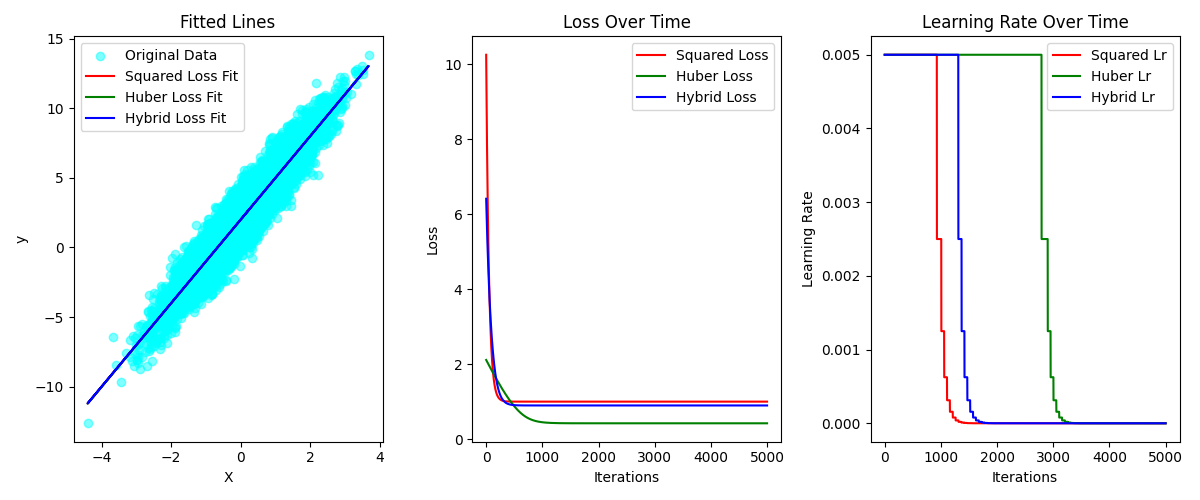
\includegraphics[width=0.8\textwidth]{assets/patience.png}
    \caption{Loss Curves for Squared, Huber, and Hybrid Losses with Modified Setup}
    \label{fig:patience_curves}
\end{figure}

\subsection{Impact of Noise Introduction}

I activated flags to introduce noise into the linear regression model (\( Y = 3X + 2 + \epsilon \)), modifying noise levels, types, and application points. Below, I address the changes and their effects, comparing results with the prior noiseless setup (5,000 steps, LR = 0.005, \( W_0 = 0.5, b_0 = 0.3 \)).

- \textbf{Noise Level Change}: Set \( \sigma_X = 0.5 \) for \( X \) and \( \sigma_Y = 2.0 \) for \( Y \), with \( \sigma_w = 0.01 \) for weights and \( \sigma_{LR} = 0.0001 \) for learning rate. Higher noise in \( Y \) (vs. \( X \)) reflects the data generation (\( \epsilon \sim \mathcal{N}(0, 2) \)), while small scales for weights and LR prevent instability.

- \textbf{Various Noise Types}: Tested Gaussian (\( \mathcal{N}(0, 1) \)), Uniform (\( U(-1, 1) \)), and Laplace (via inverse CDF). Gaussian has a bell-shaped distribution, Uniform is flat, and Laplace has heavier tails, affecting outlier frequency.

- \textbf{Noise in Data}: Added to \( X \) (\( X = X_{\text{clean}} + \text{noise}_X \)) and \( Y \) (inherent via \( \epsilon \)), increasing input/output variability.

- \textbf{Noise in Weights}: Applied Gaussian/Uniform/Laplace noise (\( \sigma = 0.01 \)) to \( W \) and \( b \) per step, simulating parameter uncertainty.

- \textbf{Noise in Learning Rate}: Added small noise (\( \sigma = 0.0001 \)) to LR, capped at \( 10^{-6} \), introducing stochastic step sizes.

- \textbf{Performance Effects}: Table~\ref{tab:noise_comparison} compares final results with the noiseless baseline. With Gaussian noise, Squared Loss rose from 1.0050 to 5.8760, Huber from 0.4274 to 1.4959, and Hybrid from 0.9027 to 3.9057, with \( W, b \) deviating from \( 3, 2 \) (e.g., Squared \( W = 2.4195 \)). Uniform noise yielded lower losses (e.g., Huber 0.7591) and closer parameters (e.g., \( W = 2.7587 \)), while Laplace noise worsened performance most (e.g., Squared 11.0941, \( W = 1.9782 \)). Noise in data raised baseline losses, weight noise slowed convergence, and LR noise with patience scheduling stabilized training but limited parameter accuracy. Huber’s robustness mitigated loss increases better than Squared’s sensitivity or Hybrid’s balance.

- \textbf{Generalizability}: In classification, Gaussian noise might blur decision boundaries, Uniform could stabilize training with fewer outliers, and Laplace might challenge robustness due to extreme values. Nonlinear models (e.g., neural networks) may amplify these effects, with weight noise acting as regularization and LR noise mimicking adaptive optimizers. However, high noise levels could disrupt convergence universally, though robust losses (e.g., Huber) may adapt better across tasks.

\begin{table}[h]
    \centering
    \caption{Comparison of Noiseless vs. Noisy Setups}
    \label{tab:noise_comparison}
    \begin{tabular}{lcccc}
        \toprule
        \textbf{Loss Function} & \textbf{Setup} & \textbf{Final Loss} & \textbf{W} & \textbf{b} \\
        \midrule
        Squared Loss & Noiseless & 1.0050 & 3.0018 & 1.9944 \\
                     & Gaussian  & 5.8760 & 2.4195 & 1.9944 \\
                     & Uniform   & 2.0366 & 2.7726 & 1.9841 \\
                     & Laplace   & 11.0941 & 1.9782 & 1.9424 \\
        Huber Loss   & Noiseless & 0.4274 & 3.0024 & 1.9924 \\
                     & Gaussian  & 1.4959 & 2.3184 & 1.8508 \\
                     & Uniform   & 0.7591 & 2.7587 & 1.9878 \\
                     & Laplace   & 2.0722 & 1.9062 & 1.6447 \\
        Hybrid Loss  & Noiseless & 0.9027 & 2.9989 & 1.9952 \\
                     & Gaussian  & 3.9057 & 2.4163 & 1.9849 \\
                     & Uniform   & 1.6074 & 2.7705 & 1.9845 \\
                     & Laplace   & 6.7979 & 1.9880 & 1.9238 \\
        \bottomrule
    \end{tabular}
\end{table}

\begin{figure}[h]
    \centering
    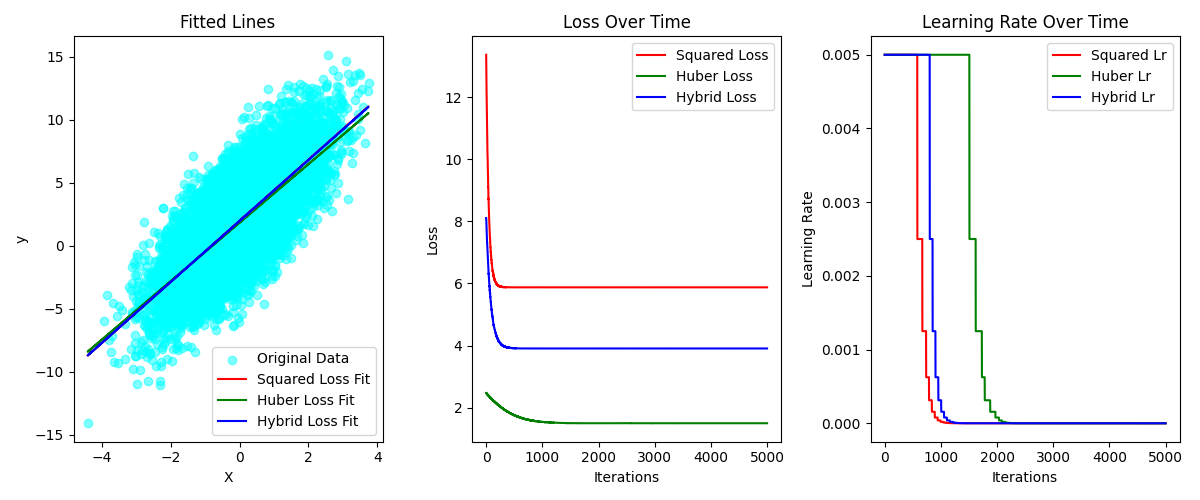
\includegraphics[width=0.8\textwidth]{assets/gaussian_noise.png}
    \caption{Gaussian Noise}
    \label{fig:gaussian_noise_curve}
\end{figure}

\begin{figure}[h]
    \centering
    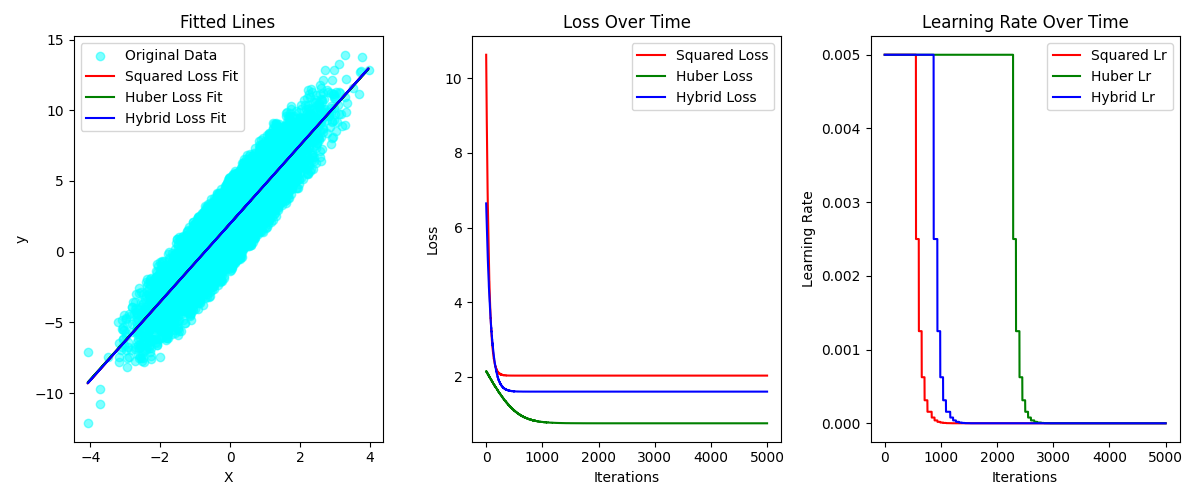
\includegraphics[width=0.8\textwidth]{assets/uniform_noise.png}
    \caption{Uniform Noise}
    \label{fig:uniform_noise_curve}
\end{figure}

\begin{figure}[h]
    \centering
    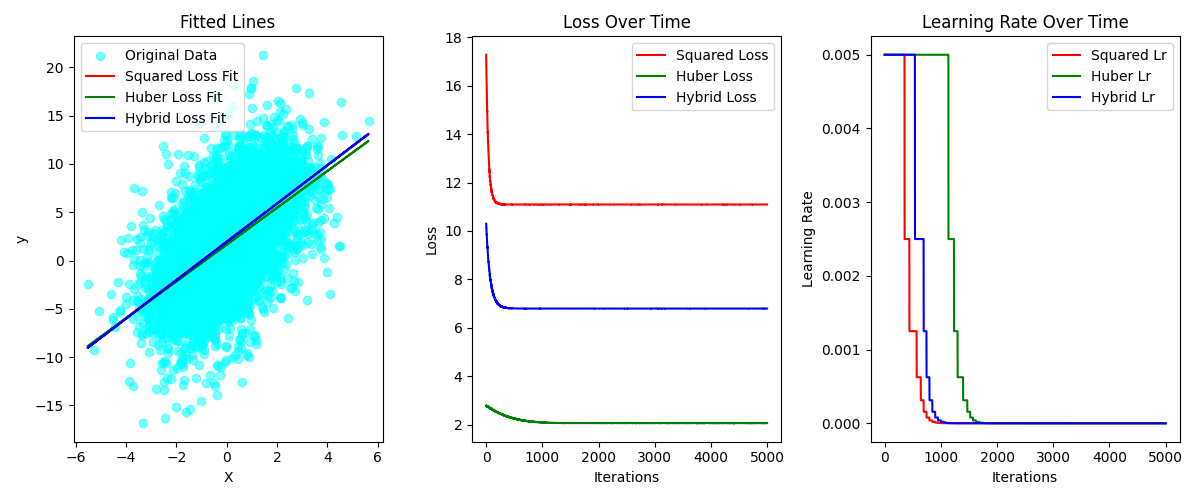
\includegraphics[width=0.8\textwidth]{assets/laplace_noise.png}
    \caption{Laplace Noise}
    \label{fig:laplace_noise_curve}
\end{figure}

\subsubsection{Robustness and Effects of Noise}

A noise-robust model is achievable, particularly with Huber loss. Its final loss rose from 0.4274 (noiseless) to 1.4959 (Gaussian), 0.7591 (Uniform), and 2.0722 (Laplace), far less than squared loss’s jump from 1.0050 to 5.8760, 2.0366, and 11.0941, respectively. Huber’s design—capping large errors—limits noise’s effect, unlike squared loss’s sensitivity or hybrid’s middle ground (0.9027 to 3.9057, 1.6074, 6.7979). Parameters stayed closer to the true \( W = 3, b = 2 \) with Uniform noise (e.g., Huber \( W = 2.7587 \)), showing robustness varies by noise type.

Noise didn’t consistently speed convergence. Gaussian noise slowed squared loss’s drop (e.g., 5.9565 at step 200 vs. 1.1627 noiseless), as did Laplace (11.1527), while Uniform was closer (2.1527). Huber converged steadily across setups (e.g., 1.6500 at step 200 with Uniform vs. 1.5618 noiseless), suggesting noise’s impact on speed depends on loss function and noise distribution, not uniformly accelerating it.

Local minima quality didn’t reliably improve. Noiseless runs hit near-optimal minima (e.g., squared loss 1.0050, \( W = 3.0018 \)), while noise raised losses (e.g., Gaussian squared 5.8760) and skewed parameters (e.g., \( W = 2.4195 \)). Uniform noise yielded better minima for Huber (0.7591 vs. 0.4274 noiseless), hinting at occasional benefits, but Laplace worsened all (e.g., squared 11.0941), indicating noise can trap models in poorer solutions.

Noise isn’t universally beneficial. It mimics real-world variability, potentially aiding generalization (e.g., Uniform’s moderate loss increase), but high levels—like Laplace’s heavy tails—degrade performance (e.g., squared loss 11.0941 vs. 1.0050). Huber’s resilience suggests noise can be managed, but for this linear task aiming at \( W = 3, b = 2 \), it generally hinders precision over the noiseless ideal.

Table~\ref{tab:noise_comparison} from the noise impact analysis supports these findings, showing Huber’s edge in robustness, variable convergence, and mixed minima outcomes.

\subsection{GPU vs. CPU Time per Epoch}

To evaluate computational efficiency, I measured the average time per training step on CPU and GPU for my model with 5,000 steps and Gaussian noise. Using a single line to enforce device usage, I tracked time across all steps for each loss function on an Intel CPU and NVIDIA GPU. Table~\ref{tab:time_comparison} presents the results.

\begin{table}[h]
    \centering
    \caption{Average Time per Step (seconds)}
    \label{tab:time_comparison}
    \begin{tabular}{lcc}
        \toprule
        \textbf{Loss Function} & \textbf{CPU Time} & \textbf{GPU Time} \\
        \midrule
        Squared Loss & 0.0044 & 0.0046 \\
        Huber Loss   & 0.0061 & 0.0063 \\
        Hybrid Loss  & 0.0054 & 0.0056 \\
        \bottomrule
    \end{tabular}
\end{table}

Surprisingly, the GPU slightly underperformed the CPU, with squared loss time rising from 0.0044s to 0.0046s, Huber from 0.0061s to 0.0063s, and hybrid from 0.0054s to 0.0056s—an increase of about 3-4\%. Device enforcement ensured consistent hardware use, verified post-run. This unexpected result likely stems from the model’s simplicity—10,000 examples and basic linear operations—where GPU overhead (e.g., data transfer) outweighs its parallelization benefits. Larger or more complex models would likely reverse this trend, favoring GPU acceleration.
\end{document}